\chapter{Interacción magnética}

\begin{miparrafo}
En temas anteriores se han estudiado varios aspectos de la Electrostática como son las fuerzas entre cargas eláctricas en reposo y su descripción en términos del campo eléctrico y del potencial. Ahora consideraremos las acciones que sufren las cargas en movimiento. Además de la fuerza representada por el campo eléctrico, una carga en movimiento puede experimentar una fuerza adicional, llamada \emph{fuerza magnética}, cuando está en presencia de otras cargas en movimiento o de imanes. Las fuerzas magnéticas también se describen convenientemente en términos de un campo vectorial -\emph{el campo magnético}- a través del cual se puede obtener la fuerza que se ejerce en cualquier punto del espacio sobre una carga en movimiento o sobre una corriente eléctrica.
\end{miparrafo}

\section{Introducción}

El origen del conocimiento de la interacción magnética hay que buscarlo varios siglos antes de Cristo, cuando el hombre observó que existen ciertos minerales de hierro, cobalto o manganeso que tienen la propiedad de atraer pequeños trozos de hierro. A esta propiedad se le dio el nombre de magnetismo. La palabra magnetismo viene de la región de Magnesia en el Asia Menor, que es uno de los lugares donde se encontraban esos materiales, en particular la \emph{magnetita}. Un material de esta clase recibe el nombre de imán, siendo el efecto más pronunciado en ciertas zonas del imán denominadas \emph{polos magnéticos}. 

La tierra actúa como un gran imán, fenómeno que se pone de manifiesto con las brújulas. La parte del imán que se alinea con el polo norte geográfico se le llama \emph{`polo norte'}, a la otra parte se le llama polo sur.

Los imanes se caracterizan porque los polos distintos se atraen y los polos iguales se repelen.

Se sospechaba que la interacción magnética tenía que ver con la eléctrica y se puso de manifiesto que matemáticamente eran proporcionales.

En el año 1600, el médico y físico ingles Willian Gilber piblica
``De magnete, magneticisque corporibus, et de magno magnete tellure'' (Sobre los imanes, los cuerpos magnéticos y el gran imán terrestre). En este trabajo Gilbert describe varias de sus experiencias con su modelo de la Tierra. A partir de los experimentos llegó a la conclusión de que la Tierra era magnética y que este era el motivo por el cual las brújulas apuntaban al norte.

A principios del s. XIX se plantea que el magnetismo es distinto a la electricidad, pues no era posible aislar los polos norte y sus de un imán pero sí se podían aislar las cargas eléctricas positivas o negativas. En 1819, el físico danés Hans Christian Orested  descubrió, de forma experimental, la relación física entre la electricidad y el magnetismo. Era profesor en la universidad de Copenhague y, un día, antes de dar su clase realizó el siguiente experimento:

\begin{figure}[H]
	\centering
	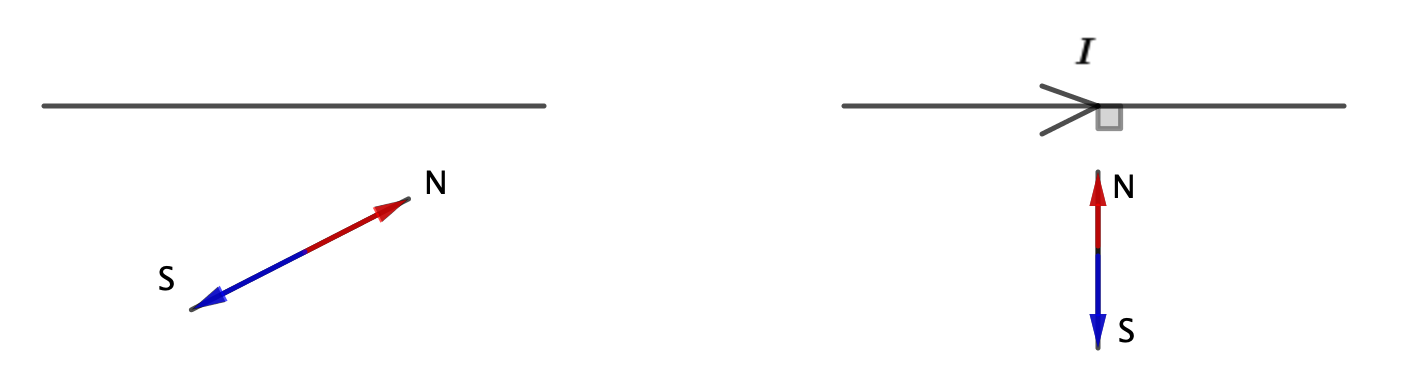
\includegraphics[width=.9\textwidth]{imagenes/imagenes26/T26IM01.png}
\end{figure}

Cuando por un cable eléctrico circula corriente de intensidad $I$, la aguja de la brújula se orienta perpendicularmente al cable.

Más tarde, Ampère interpretó el experimento de Orested y los trabajos de faraday pudieron establecer una teoría del magnetismo.

\section[Equivalencia entre imanes y corrientes. Campo magnético. Ley de Ampère-Laplace]{Equivalencia entre imanes y corrientes. Campo magnético. Ley de Ampère-Laplace\sectionmark{Campo magnético}}
\sectionmark{Campo magnético}
Experiencias:

\begin{enumerate}
\item Un hilo por el que circula corriente eléctrica altera su espacio circundante de manera que manera que una aguja imantada se pone perpendicular a la corriente, invirtiéndose el sentido de orientación de la aguja si se invierte el sentido de la corriente.
\item Si se sustituye la aguja imantada por una bobina por la que circula corriente, la bobina se comporta del mismo modo que la aguja imantada. Si se interrumpe la corriente no se observa fenómeno alguno.
\item Cuando se coloca junto al hilo conductor una carga eléctrica estática y se conecta la corriente en el hilo conductor, no se observa fenómeno alguno.
\item Cuando se acercan dos hilos conductores por los que circula corriente alteran sus posiciones acercándose o alejándose según las corrientes en los hilos tengan el mismo sentido o sentidos contrarios. La interacción es tanto mayor cuanto lo sea la intensidad que circula por los conductores y cuanto menor sea la distancia que los separa. Si se interrumpe la corriente en alguno de los dos hilos conductores, el fenómeno deja de observarse.
\end{enumerate}

Consecuencias:

\begin{enumerate}
\item Existen \colorbox{LightYellow}{equivalencias entre imanes y corrientes}, ambos alteran su espacio circundante de identica forma, toman la misma orientación
\item Como un hilo por el que no circula corriente eléctrica no sufre alteración, \colorbox{LightYellow}{la interacción se produce en cargas en movimiento}, es decir, si hay corriente.
\item Si imanes y corrientes eléctricas son equivalentes, cabe pensar\colorbox{LightYellow}{los imanes} \colorbox{LightYellow} {deben sus propiedades a corrientes eléctricas interiores}, corrientes moleculares. (Idea sugerida por Ampère).
\end{enumerate}

De todas estas experiencias se pudo construir una expresión matemática que explica muy bien los hechos detectados experimentalmente.

\begin{multicols}{2}
$$\dd \vec F_{12}=k_m\dfrac{I_1I_2\dd \vec l_1 \times (\dd \vec l_2 \times \vec u_r)}{r^2}$$

$\quad$
\begin{figure}[H]
	\centering
	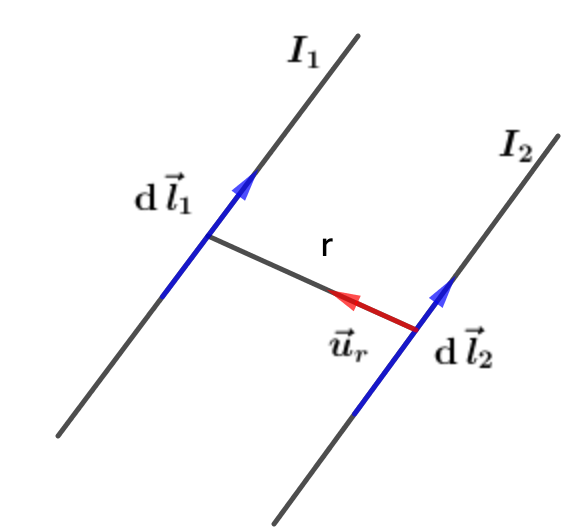
\includegraphics[width=.35\textwidth]{imagenes/imagenes26/T26IM02.png}
\end{figure}	
\end{multicols}

$k_m$ es la constante de proprcionalidad, en el $SI$ tiene un valor y se expresa en $k_m=10^{-7}\ \mathrm{m\ kg\ C}^{-2}$. 

Es más útil la expresión $k_m=\dfrac{\mu_0}{4\pi}$ con $\mu_0$ la llamada \emph{permeabilidad magnética del vacío} cuyo valor es 
$\mu_0 = 4 \pi \times 10^{-7} \ \mathrm{m\ kg\ C}^{-2}$ y la ley experimental del magnetismo se escribirá como:

\begin{equation}
\dd \vec F_{12}=\dfrac{\mu_0}{4\pi} \dfrac{I_1I_2\dd \vec l_1 \times (\dd \vec l_2 \times \vec u_r)}{r^2}	
\end{equation}

Reordenando, $\ \dd \vec F_{12}=
I_1 \dd \vec l_1 \times \left[ 
\dfrac{\mu_0}{4\pi} I_2 \dfrac{\dd \vec l_2 \times \vec u_r}{r^2}
\right]$	

A la parte entre corchetes, que es característica del segmento diferencial y de la distancia de separación de cables, le llamamos \emph{campo magnético},

$\dd \vec B_2=\dfrac{\mu_0}{4\pi} I_2 \dfrac{\dd \vec l_2 \times \vec u_r}{r^2}$, campo magnético elemental creado por el segundo elemento diferencial. Así,

\begin{equation}
\boldsymbol{ \dd \vec F_{12} \ = \ I_1 \ \dd \vec l_1 \ \times \ \dd \vec B_2 } \qquad \ 1^a \ \textbf{Ley de Laplace}	
\end{equation}
\vspace{35mm}%************************************************
\begin{multicols}{2}
$\quad$

En el caso de un circuito, el campo magnético será:

\begin{figure}[H]
	\centering
	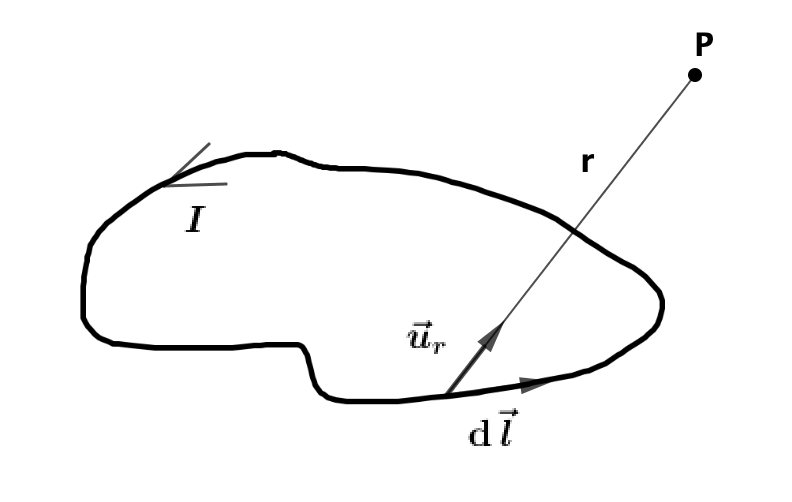
\includegraphics[width=.3\textwidth]{imagenes/imagenes26/T26IM03.png}
\end{figure}	
\end{multicols}

\begin{equation}
\boldsymbol{ \vec B \ =\ \dfrac {\mu_0}{4\pi} \ \oint \  I \ \dfrac {\dd \vec l \times \vec u_r}{r^2} }  \qquad \textbf{Ley de Ampère-Laplace}	
\end{equation}

En el $SI$, $\ [B]=\mathrm{kg\ s}^{-1}\ \mathrm{C}^{-1}$ y su unidad recibe el nombre de \emph{miriagauss, Tesla o Webber/m$^2$}. Un miriagauss son $10^4$ gauss.

\subsection{Campo magnético creado por una carga móvil}

\begin{multicols}{2}
$\quad \dd \vec B=$

$\quad =\dfrac{\mu_0}{4\pi} I \dfrac{\dd \vec l \times \vec u_r}{r^2} = $

$\quad =\dfrac {\mu_0}{4\pi} \dfrac{\dd q}{\boldsymbol{ \dd t}} \dfrac{\boldsymbol{ \dd \vec l }\times \vec u_r}{r^2}=$

$\quad = \dfrac {\mu_0}{4\pi} \dd q \dfrac{\boldsymbol{\vec v} \times \vec u_r}{r^2}$
	\begin{figure}[H]
	\centering
	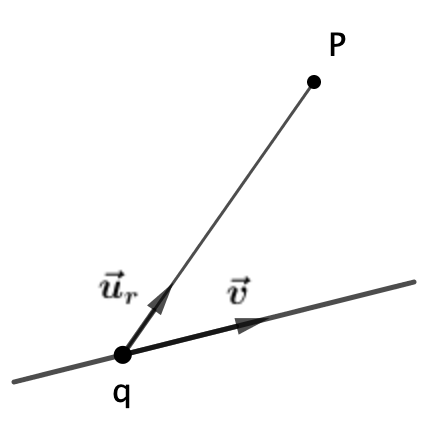
\includegraphics[width=.3\textwidth]{imagenes/imagenes26/T26IM04.png}
	\end{figure}	
\end{multicols}

Integrando, 

\begin{equation}
\vec B \ = \ \dfrac{\mu_0}{4\pi} \ q \ \dfrac {\vec v \times \vec u_r}{r^2}	
\end{equation}

Si la carga no se mueve, $\vec v=0$, entonces no hay campo magnético, $\vec B=0$.

Comparando con el campo eléctrico creado por una carga puntual (ec. \ref{campo-electrico-carga-puntual}), tenemos

\begin{equation}
\subrayado{ \  \boldsymbol {\vec B=} \ 	} \mu_0 \ \varepsilon_0 \ \vec v \times \vec E \ = \  \subrayado{ \  \boldsymbol{ \  \dfrac 1 {c^2} \ \vec v \times \vec E }  \ }
\end{equation}

El producto de las dos constantes universales $\varepsilon_0 \text{ y } \mu_0$ tiene dimensiones de $[v^{-2}]$. 
$\quad \dfrac 1 {\sqrt{\mu_0 \ \varepsilon_0} } = \ c \ = 3\times 10^8\ \mathrm{m\ s}^{-1}$

\subsection{Campo magnético de una corriente rectilínea. Ley de Biot-Savart}

\begin{multicols}{2}

$\quad$

$\dd \vec B=\dfrac{\mu_0}{4\pi} I \dfrac{\dd \vec l \times \vec u_r}{r^2} $

$\quad$

En $P$, $\dd \vec B$ es perpendicular al plano de la imagen. $\vec B$ será siempre tangente a la circunferencia que pasa por $P$, de radio $R$ y sentido el de avance de un sacacorchos.
	\begin{figure}[H]
	\centering
	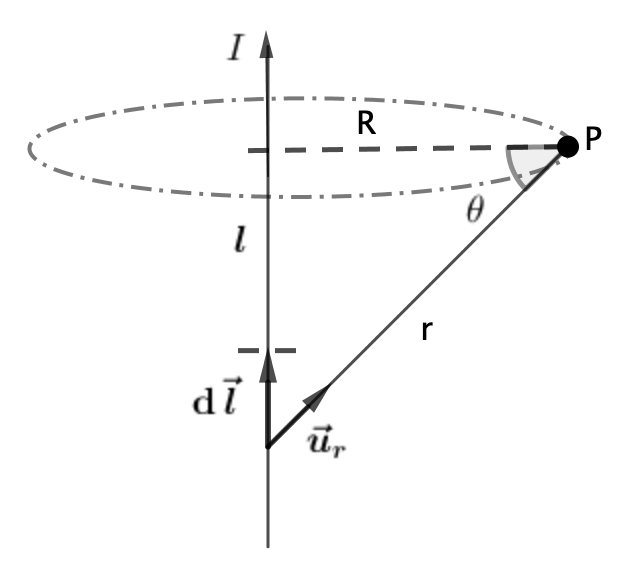
\includegraphics[width=.4\textwidth]{imagenes/imagenes26/T26IM05.png}
	\end{figure}	
\end{multicols}

$\dd B=\dfrac{\mu_0}{4\pi} I \dfrac{\dd l \sin \theta}{r^2};\qquad l=R\tan \theta; \quad \dd l=\dfrac {R}{\cos^2 \theta} \dd \theta; \quad r=\dfrac {R}{\cos \theta}$

$\dd B= \dfrac {\mu_0}{4\pi} I \dfrac{R \dd \theta}{\cos^2 \theta} \dfrac {\sin \theta}{\dfrac{R^2}{\cos^2 \theta}}= \dfrac {\mu_0}{4\pi} \dfrac I R \sin \theta \dd \theta$

Integrando, $\ \displaystyle B= \dfrac {\mu_0}{4\pi} \dfrac I R \int_{-\pi/2}^{\pi/2} \sin \theta \dd \theta =  \dfrac {\mu_0}{4\pi}  \dfrac I R 
\cancelto{2}{
\left[ \cos \theta \right]_{-\pi/2}^{\pi/2}}$




\begin{equation}
	\subrayado{ \ \boldsymbol{ B \ = \ \dfrac {\mu_0 \ I}{2 \pi R} } \ }	\qquad \textbf{Ley de Biot-Savart}
\end{equation}

En una corriente rectilínea, las líneas del campo magnético son circunferencias concéntricas y el campo magnético siempre es tangente a estas circunferencias. El sentido del campo lo da la \emph{`regla de la mano derecha': usando el pulgar de la mano derecha para indicar el sentido de la intensidad de corriente, los dedos restantes indicarán el sentido del campo magnético.}


\begin{figure}[H]
	\centering
	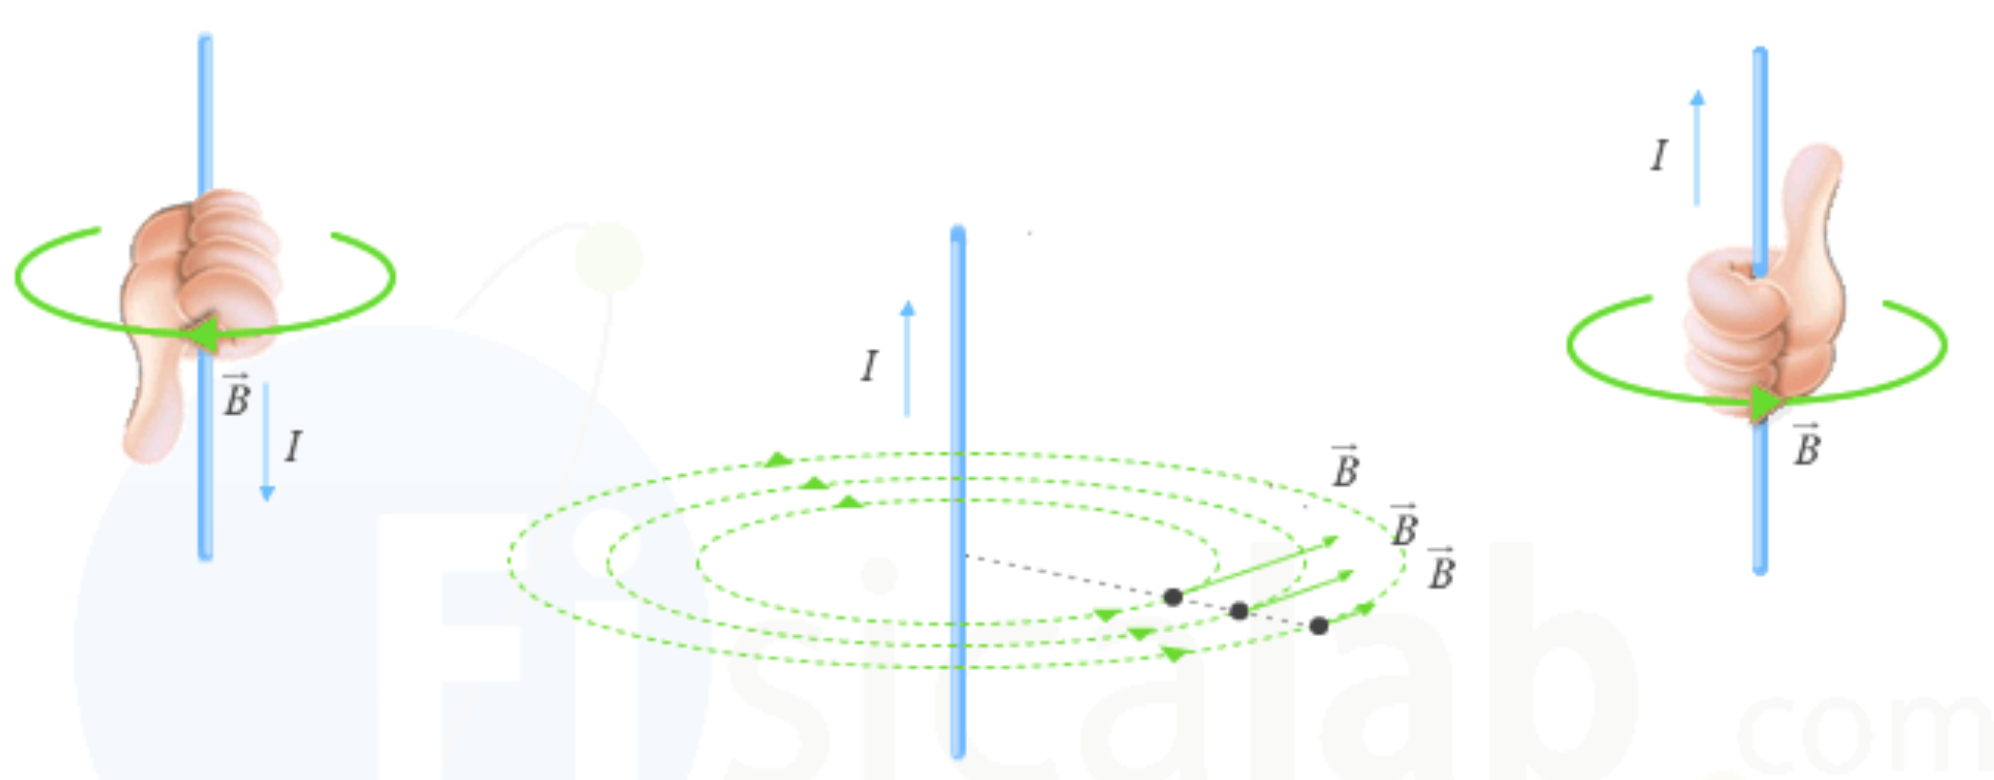
\includegraphics[width=.8\textwidth]{imagenes/imagenes26/T26IM07.png}
	\end{figure}

\subsection{Campo magnético en el eje de una corriente circular}

Recordemos: $\ \dd \vec F_{12}=I_1 \dd \vec l_1 \times \dd \vec B;\qquad  \dd \vec B=\dfrac {\mu_0}{4\pi} I \dfrac {\dd \vec l \times \vec r}{r^2}$

\begin{figure}[H]
	\centering
	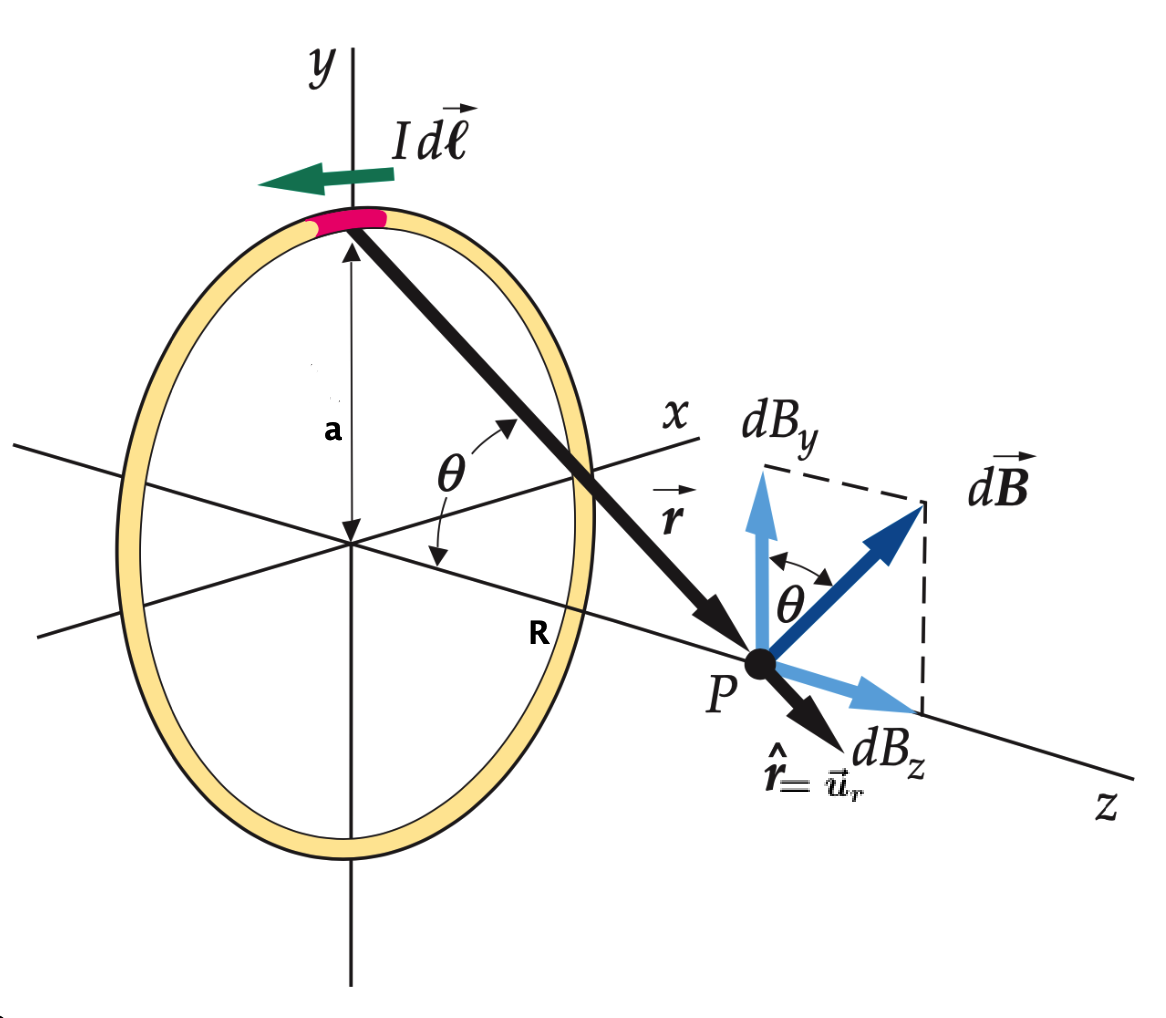
\includegraphics[width=.75\textwidth]{imagenes/imagenes26/T26IM06.png}
	\end{figure}


$\vec u_r \ \bot \ \dd \vec l; \quad \dd B =\dfrac{\mu_0}{4\pi}I\dfrac{\dd l}{r^2};\quad B=\displaystyle \oint \dd B_x =\oint \dd B \sin \theta$

$\displaystyle B=\oint \dfrac{\mu_0}{4\pi} I \dfrac{\dd l}{r^2} \sin \theta ; \quad \oint \dd l =2\pi a, $ longitud de la circunferencia.

$\subrayado{\ \boldsymbol{B\ =} \ } \ \dfrac{\mu_0}{4\pi} \ I \  \dfrac {2\pi a}{r^2} \ \sin \theta = \ \textcolor{gris}{\left[ \sin \theta = \dfrac a r \right]} \ =
\subrayado{ \ \boldsymbol{\dfrac{\mu_0\ I}{2} \ } \ \dfrac {a^2}{r^3}} ; \quad \textcolor{gris}{(\ r^2=R^2+a^2 \ )}$


\begin{equation}
\subrayado{\ \boldsymbol{B \ = \ \dfrac{\mu_0\ I}{2} \ \dfrac{a^2}{(R^2+a^2)^{3/2}} } \ }	
\end{equation}

Cuando $R=0$, esta ecuación nos proporciona el \textsf{campo magnético en el centro de la espira}, $\subrayado{\boldsymbol{ B=\dfrac{\mu_0 I}{2a}}}$

En una corriente circular (espira), las líneas del campo magnético son circunferencias concéntricas y el campo es siempre tangente a cualquier punto de esas circunferencias.. El sentido del campo lo da la \emph{`regla de la mano derecha': si el pulgar de la mano derecha indica el sentido de la intensidad de corriente, los dedos indicarán el sentido del campo magnético}.

\begin{figure}[H]
	\centering
	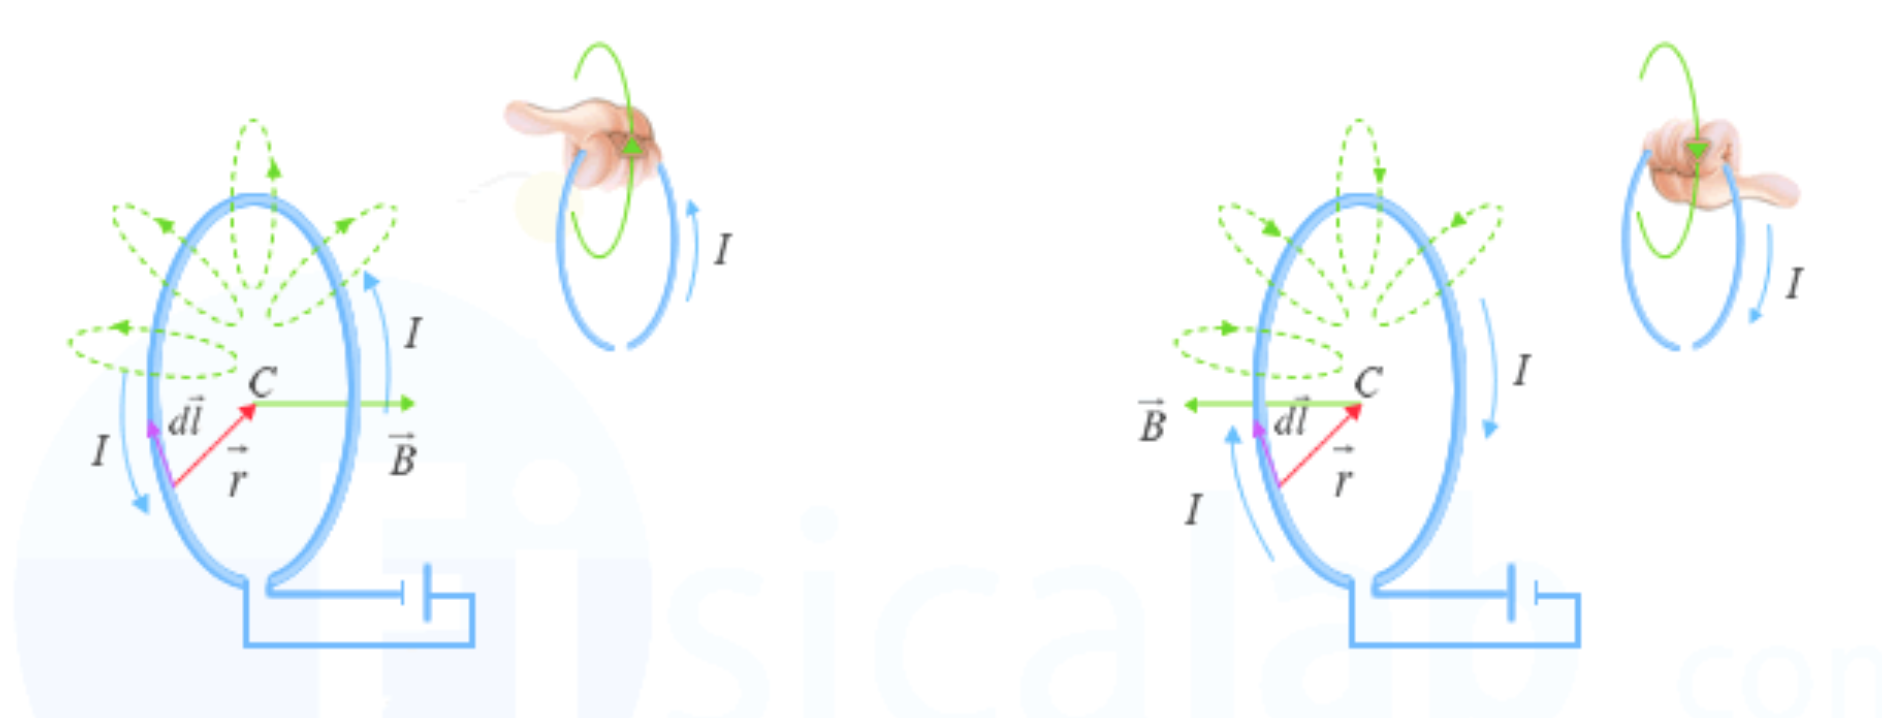
\includegraphics[width=1\textwidth]{imagenes/imagenes26/T26IM08.png}
	\end{figure}

Nota: las imágenes del sentido del campo de esta subsección y la anterior son de ``\textsf{https://www.fisicalab.com/apartado/campo-magnetico-creado-corriente-electrica}.''

\subsection{Campo magnético en un punto del eje de una corriente solenoidal.}

Un solenoide es un hilo conductor formado por bobinas, cada una de las cuales es aproximadamente una espira.

\begin{multicols}{2}
$N=$ número de espiras.

$\dfrac N L = cte$

$\dd N=\dfrac N L \dd x$

$I$ es la corriente que circula por el solenoide; $I\dd N$ es la cantidad de intensidad que circula por $\dd x$
\begin{figure}[H]
	\centering
	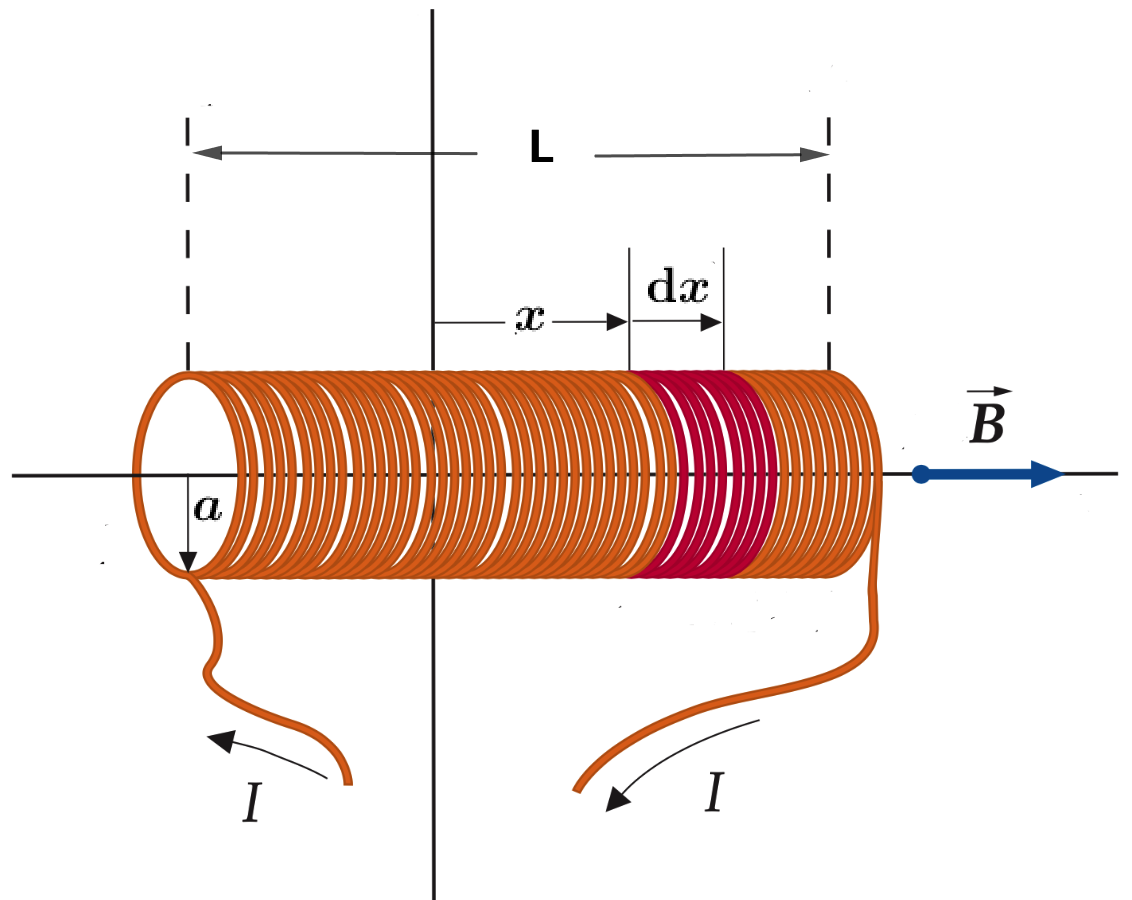
\includegraphics[width=.4\textwidth]{imagenes/imagenes26/T26IM09.png}
	\end{figure}	
\end{multicols}

\vspace{-5mm}%************************************************

$ I \ \to \ I \dd N=I\dfrac N L \dd x$

$\dd B$ de una espira, por la subsección anterior, ser-a:

$\dd B=\dfrac{\mu_0}{2} \dfrac{a^2}{r^3} I \dfrac N L \dd x$

Las magnitudes variables en esta expresión son $x$ y $r$. Interpretémoslas en función de una tercera variable.

\begin{multicols}{2}
$\dd l=r \dd \theta$

$\dd x=\dfrac {\dd l}{\cos(90^o-\theta)}=\dfrac {\dd l}{\sin \theta}$

$\dd B=\dfrac {\mu_0 I N}{2L} \sin \theta \dd \theta$ 
\begin{figure}[H]
	\centering
	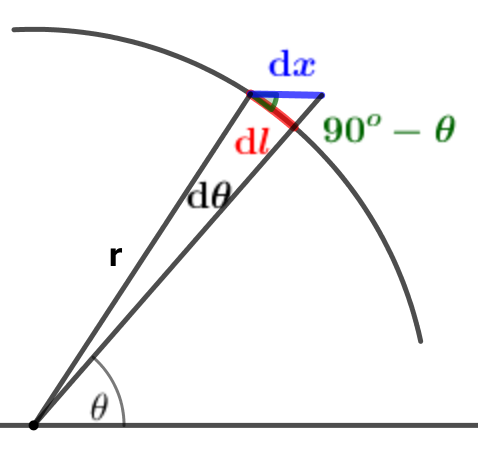
\includegraphics[width=.2\textwidth]{imagenes/imagenes26/T26IM10.png}
	\end{figure}	
\end{multicols}

Integrando, $\ \displaystyle B=\dfrac {\mu_0 I N}{2L} \int_{\theta_1}^{\theta_2} \sin \theta \dd \theta=-\dfrac {\mu_0 I N}{2L} [\cos \theta]_{\theta_1}^{\theta_2}$

\begin{equation}
\boldsymbol{	B \ = \ \dfrac {\mu_0 I N}{2L} \ (\cos \theta_1 - \cos \theta_2) }
\end{equation}

Un caso interesante es el solenoide muy largo, $\dfrac a L << 1$, $\theta_1\to 0;\ \theta_2 \to \pi$. El campo, en el centro del solenoide vale:

\begin{equation}
\subrayado{ \ \boldsymbol{B\ = \  \dfrac{\mu_0IN}{L} }	\ }\ ; \qquad \bold{B} \textbf{ en centro solenoide muy largo}
\end{equation}

Sobre el eje del solenoide muy largo y en uno de sus extremos, $\theta_1\to 0;	 \theta_2\to \pi/2$

\begin{equation}
\subrayado{ \ \boldsymbol{B\ = \  \dfrac{\mu_0IN}{2L} }	\ }\ ; \qquad \bold{B} \textbf{ en extremo solenoide muy largo}
\end{equation}

$B$ en el centro de un solenoide muy largo es sobre que en sus extremos. Hay un `gradiente' de B en el eje del solenoide, hay variación de $B$ respecto al centro del solenoide a medida que nos alejamos de él.

\section[Fuerzas magnéticas en distintos elementos de corriente]{Fuerzas magnéticas en distintos elementos de corriente{\sectionmark{Fuerzas magnéticas. Casos}}}
\sectionmark{Fuerzas magnéticas. Casos}

Recordemos la primera ley de Laplace:
$\quad \boldsymbol{ \dd \vec F_{12} \ = \ I_1 \ \dd \vec l_1 \ \times \ \dd \vec B_2 }$

En general, $\boldsymbol{ \dd \vec F = I \dd \vec l \times \vec B }$, donde $\vec B$ es la resultante, en el punto considerado, de todos los elementos del universo que crean campo magnético. Esta es la \textbf{ley de Laplace}.

\subsection{Fuerza magnética sobre una carga en movimiento. Efecto Hall}

Consideremos una carga $\dd q$ en movimiento, pasado un tiempo $\dd t$, la carga se desplaza una distancia $\dd \vec l$, con $\vec v=\dv{\vec l}{t}$.

$\dd \vec F=I\dd \vec l \times \vec B=\displaystyle \dv{q}{t} \dd \vec l \times \vec B = \dd q \vec v \times \vec B$

Integrando para toda la carga,

\begin{equation}
	\subrayado{\ \boxed{\ \boldsymbol{\vec F \ = \ q\ \vec v \times \vec B} \ } \ } \qquad \textbf{Fuerza de Lorentz}
\end{equation}

\textbf{Efecto Hall:} aparición de un potencial eléctrico debido a la fuerza de Lorentz sobre una corriente.

Si una corriente eléctrica fluye a través de un conductor situado en un  campo magnético, éste campo ejerce una fuerza transversal sobre los portadores de cargas móviles, que tiende a empujarlas hacia un lado del conductor. Esto es más evidente en un conductor plano delgado como el mostrado. La acumulación de cargas en los lados del conductor, equilibrará esta influencia magnética, produciendo un voltaje medible entre los dos lados del conductor. La presencia de este voltaje transversal medible se llama efecto Hall en honor de E. H. Hall que lo descubrió en 1879. 

Note que la dirección de la corriente I en el diagrama es la de la corriente convencional, de modo que el movimiento de electrones es en la dirección opuesta. Eso confunde aún mas todas las manipulaciones de la `regla de la mano derecha’ que debemos realizar para obtener las direcciones de las fuerzas.

\begin{figure}[H]
	\centering
	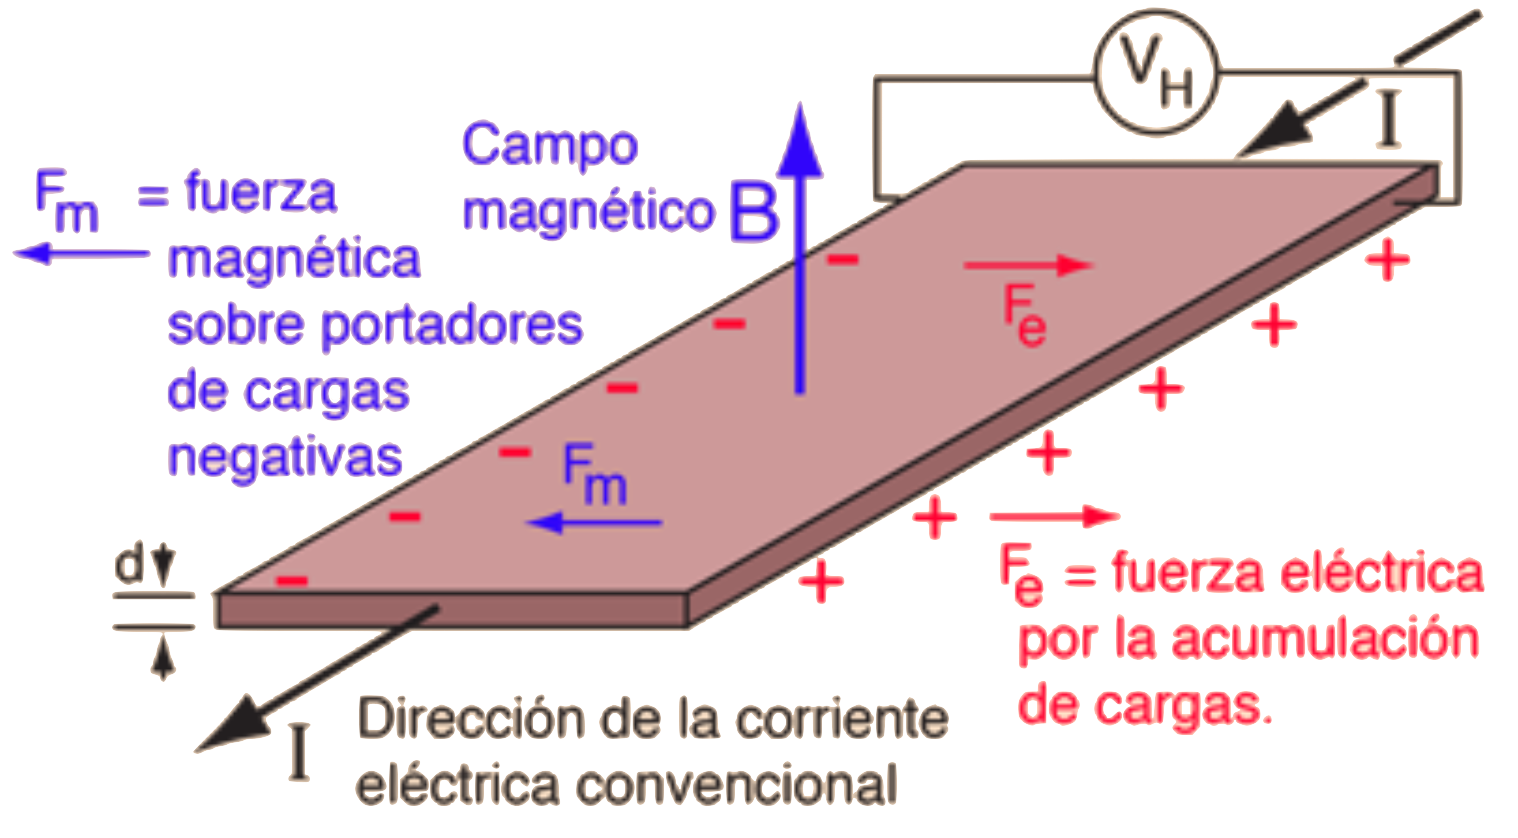
\includegraphics[width=.9\textwidth]{imagenes/imagenes26/T26IM11.png}
	\end{figure}

$F_m$ es la fuerza magnética sobre la carga en movimiento, fuerza de Lorents.  Aparece un campo eléctrico debido al exceso de cargas positivas y negativas en los extremos del conductor que da lugar a una fuerza eléctrica, $F_e$. La fuerza de Lorentz sobre las partículas cargadas que circulan por una lámina conductora genera un potencial eléctrico debido a la acumulación de cargas en los bordes de ésta.

\begin{figure}[H]
	\centering
	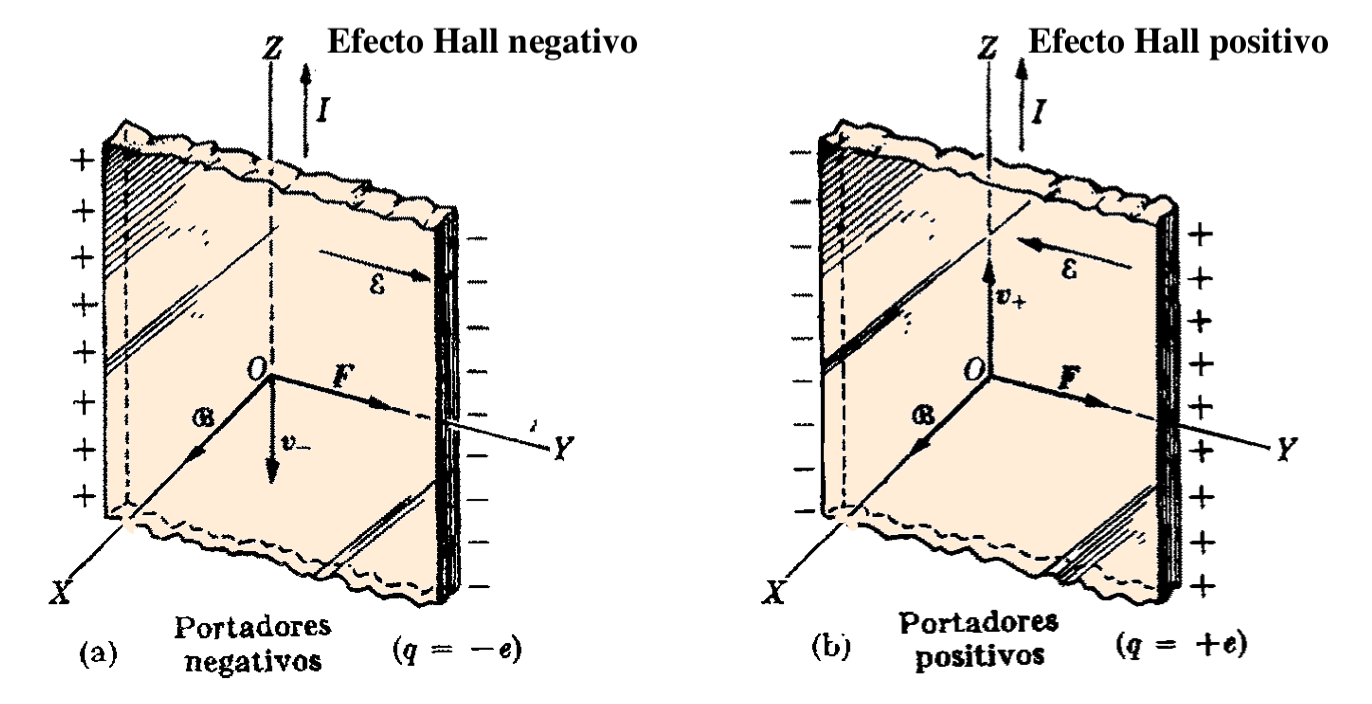
\includegraphics[width=.9\textwidth]{imagenes/imagenes26/T26IM12.png}
	\end{figure}

Existen dos tipos de efectos Hall, el negativo (cobre, oro, plata, platino) y el positivo (Cobalto y Cinc), Hall lo descubrió más tarde.

La polarización depende de si las cargas que se están moviendo son positivas o negativas. En los conductores, lo que se desplazan son electrones, por lo que la situación coincide con la representada en la figura a). Por el contrario, hay algunos `semiconductores' donde tiene lugar una corriente de `huecos', es \emph{como si} e tratase de cargas positivas en movimiento. El signo del potencial permite conocer el tipo de portador.

\subsection{Fuerza magnética sobre una corriente eléctrica rectilínea}

$\dd \vec F  = I\dd \vec  l \times \vec B=I\dd l \vec u_l \times \vec B$

Fuerza por unidad de longitud del conductor, $\ \displaystyle \dv{\vec F}{l} = I\vec u_l \times \vec B$

En el caso particular en que $\vec B=\overrightarrow{cte}$ si se puede calcular la fuerza, dando como resultado:

$\vec F = I \vec L \times \vec B$

Como caso particular, veamos la \textbf{fuerza entre corrientes rectilíneas paralelas}:

\begin{figure}[H]
	\centering
	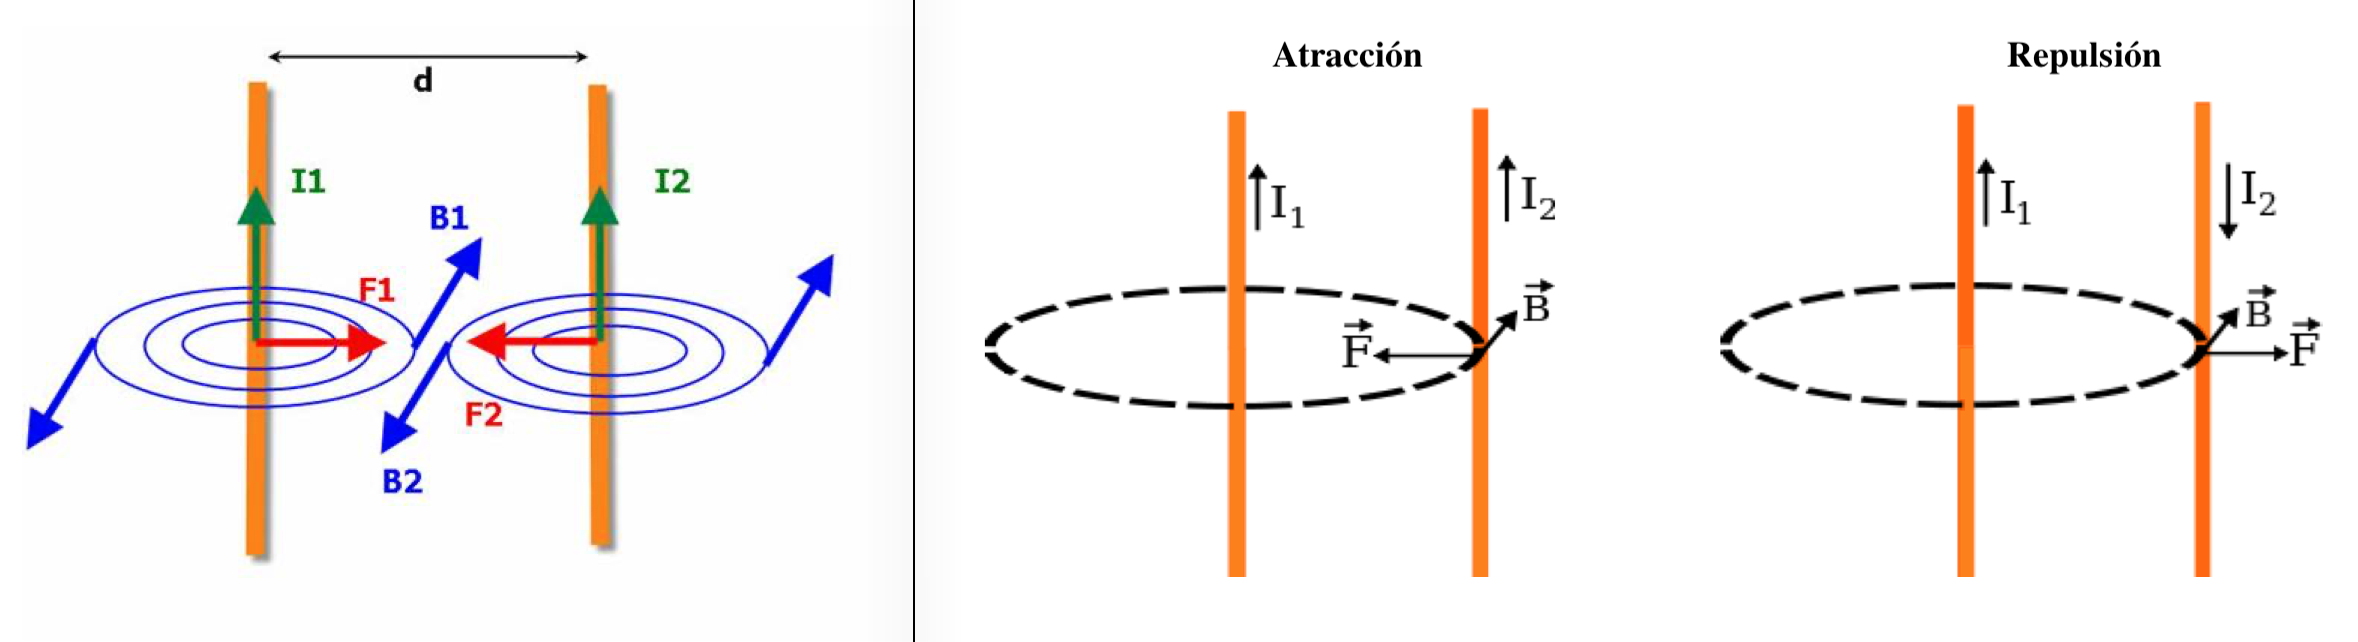
\includegraphics[width=1\textwidth]{imagenes/imagenes26/T26IM13.png}
	\end{figure}

\begin{figure}[H]
	\centering
	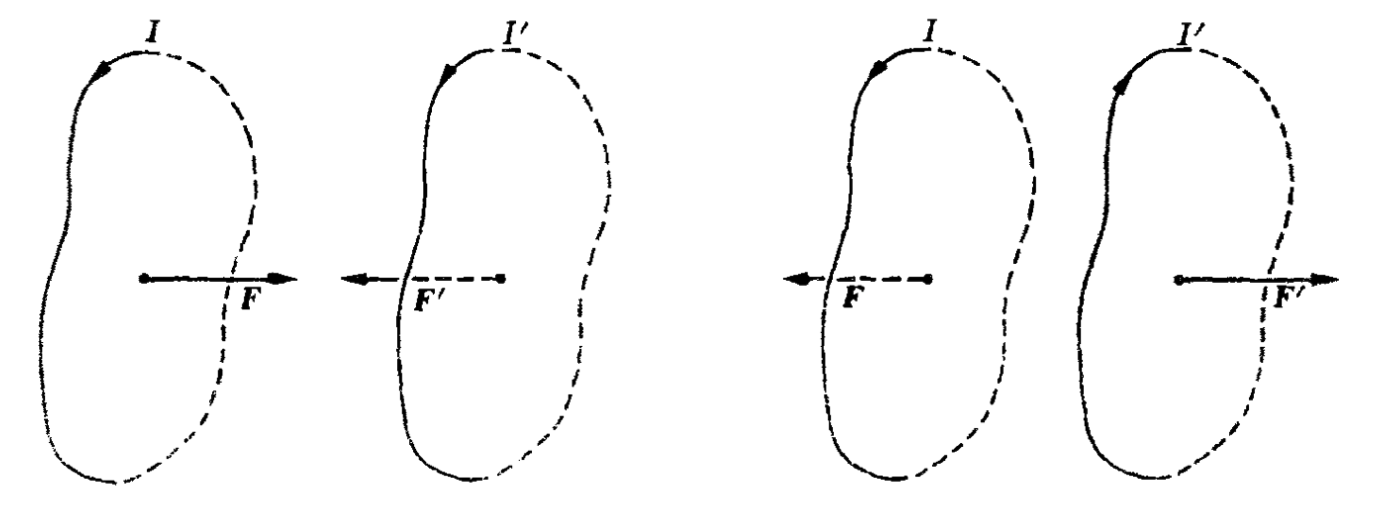
\includegraphics[width=.9\textwidth]{imagenes/imagenes26/T26IM15.png}
	\end{figure}

$B=cte \quad B\ = \ \dfrac {\mu_0\ I}{2 \pi \ d} \qquad \text{Ley de Biot-Savart} $

Según la ley de Laplace, $\ \dd \vec F= I_2 \dd \vec l_2 \times \dfrac{\mu_0 I}{2 \pi r}\vec u:c$, 

donde $r$ distancia del cable $I_2$ y $\vec u_c$ vector perpendicular a la circunferencia.

$\dd \vec F=I_1I_2 \dfrac{\mu_0}{2 \pi} \dfrac{\dd \vec l \times \vec u_c}{r};\qquad \dd \vec l=\dd l \vec u_l;\quad \vec u_l \times \vec u_c=\vec u_r$

Dos corrientes rectilíneas paralelas , separadas una distancia $d$, recorridas por corrientes en el mismo sentido se atraen con la fuerza:

\begin{equation}
\subrayado{\ \boldsymbol{\dv{F}{l}\ = \ I_1\ I_2\ \dfrac{\mu_0}{2\pi} \dfrac 1 d} \ } 	
\end{equation}

Si las corrientes circulan en sentidos contrarios la fuerza es la misma pero ahora es repulsiva.



Esto nos permite definir el ampère como unidad fundamental.



\begin{myexampleblock}{Notación sobre unidades}
	Son magnitudes sundamentales: $[L],\ [M], [T]$ cuyas unidades en el $SI$ son $\mathrm{m},\ \mathrm{kg},\ \mathrm{s}$.
	Definimos también la carga eléctrica: $\ [Q] \ \to \ \mathrm{C}$
	
 	$$\begin{cases}
\ \text{Ley Coolomb} \quad & 	\ F=K_e \dfrac{q_1q_2}{r^2}\\
\ \text{Ampère y Orested} & \ F2=k_m \dfrac{I_1 I_2}{r} 
\end{cases}
 $$
 
\vspace{2mm} Eligiendo arbitrariamente una de las unidades Coulomb o Ampère, la otra queda supeditada a ésta. En $SI,\quad \mu_0\varepsilon_0=1/c^2$.
 
\vspace{2mm} Experimentalmente es más sencillo determinar la fuerza entre corrientes que entre cargas. Por ello se eligió tomar el ampère como unidad fundamental y el coulomb como derivada.
 
\vspace{2mm} \emph{Se define el \textbf{ampère} como la corriente que circula por dos c0nductores rectilíneos y paralelos separados $1\ \mathrm{m}$ de longitud que produce una fuerza de atracción sobre los conductores de $2\times 10^{-7} \ \mathrm{N\ m}^{-1}$}.
 
\vspace{2mm} Ahora, \emph{el \textbf{coulomb} es la carga que pasa durante $1\ \mathrm{s}$ por una sección transversal de un conductor cuya intensidad es de $1\ \mathrm{A}$.}
\end{myexampleblock} 



\section{Momento dipolar magnético}

\begin{multicols}{2}
Circuito de corriente cuadrangular de dimensiones $L$ y $L'$ por done circula una intensidad $I$ y en presencia de un campo magnético uniforme $B$ perpendicular al circuito.

Respecto de los lados $L$: 

$\vec F = I \vec L \times \vec B$, ley de Ampère-Laplace.

Respecto de los lados $L'$: 

$\vec F = I \vec L' \times \vec B$,

$\vec u_N$ vector unitario que representa a la superficie del circuito y lleva el sentido del avance de un sacacorchos que gire en el sentido de la intensidad de corriente.
\begin{figure}[H]
	\centering
	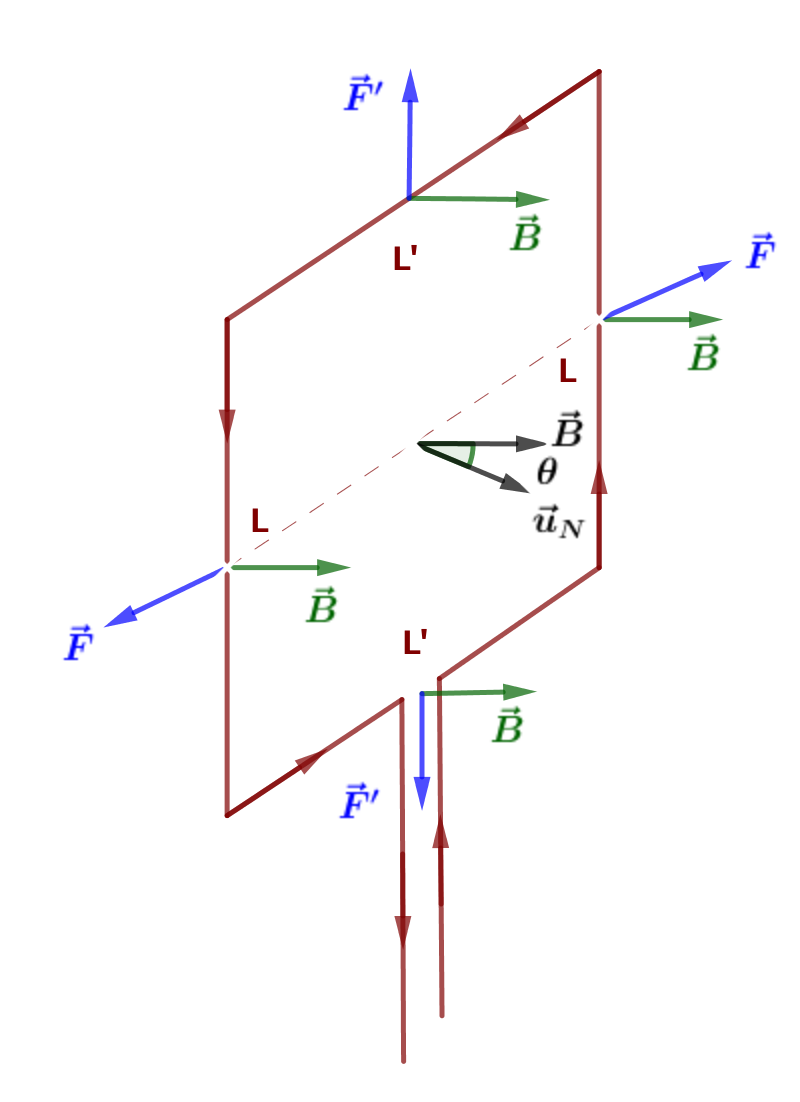
\includegraphics[width=.4\textwidth]{imagenes/imagenes26/T26IM14.png}
	\end{figure}	
\end{multicols}

Las fuerzas $\vec F'$ tienen sentidos contrarios pero al estar en la misma recta, dan lugar a una deformación del circuito hacia arriba y hacia abajo.

Las fuerzas $\vec F$ tienen sentidos contrarios dan lugar a un par de fuerzas cuyo valor, en módulo, es: $M=ILB\ L'\sin \theta=ISB\sin \theta$

Si definimos $\subrayado{ \ \boldsymbol{\vec m = I \ \vec S = I \ S \ \vec u_n}\ } $

\begin{equation}
\subrayado{\ \boldsymbol{ \vec M \ = \ \vec m \times \vec B	} \ }
\end{equation}


La magnitud $\ \vec m \ $ recibe el nombre de \emph{``momento dipolar magnético''}, se ha definido como el producto de la intensidad del circuito por su vector superficie.

$[\vec m]=\mathrm{C\ T}^{-1} \mathrm{M}^2$, en el $SI$ se mide en $\mathrm{A\ m}^{-2}$

La ecuación del momento dipolar magnético $\vec M=\vec m \times \vec B$ guarda analogía formal con la del momento dipolar eléctrico, $\vec M=\vec p \times \vec E$. Poer ello, así com $\mathcal E_p (\text{eléctrica}) = - \vec p \cdot \vec E,\ $ ahora $\ \boldsymbol{\mathcal E_p(\text{magnética})=-\vec m \cdot \vec B}$

\begin{miparrafodestacado}
Consecuencia: nuestro dipolo magnético (circuito cuadrangular) girará hasta alcanzar el equilibrio que se conseguirá cuando  la orientación sea paralela al campo, $\ \vec m \ || \ \vec B$.	
\end{miparrafodestacado}


\begin{multicols}{2}
Si los imanes están constituidos por corrientes cerradas, cada una de estas corrientes cerradas tendrá asociada un momento dipolar magnético por lo que el propio imán tendrá su momento dipolar magnético que será el responsable de que el imán se oriente (aguja imantada de la brújula).

Tambén explica este hecho que la espira y es solenoide tengan momentos dipolares magnéticos: $\vec m_e=I\ \vec S_e$, $\ \vec m_s=N_e \ I\ \vec S_e$.
\begin{figure}[H]
	\centering
	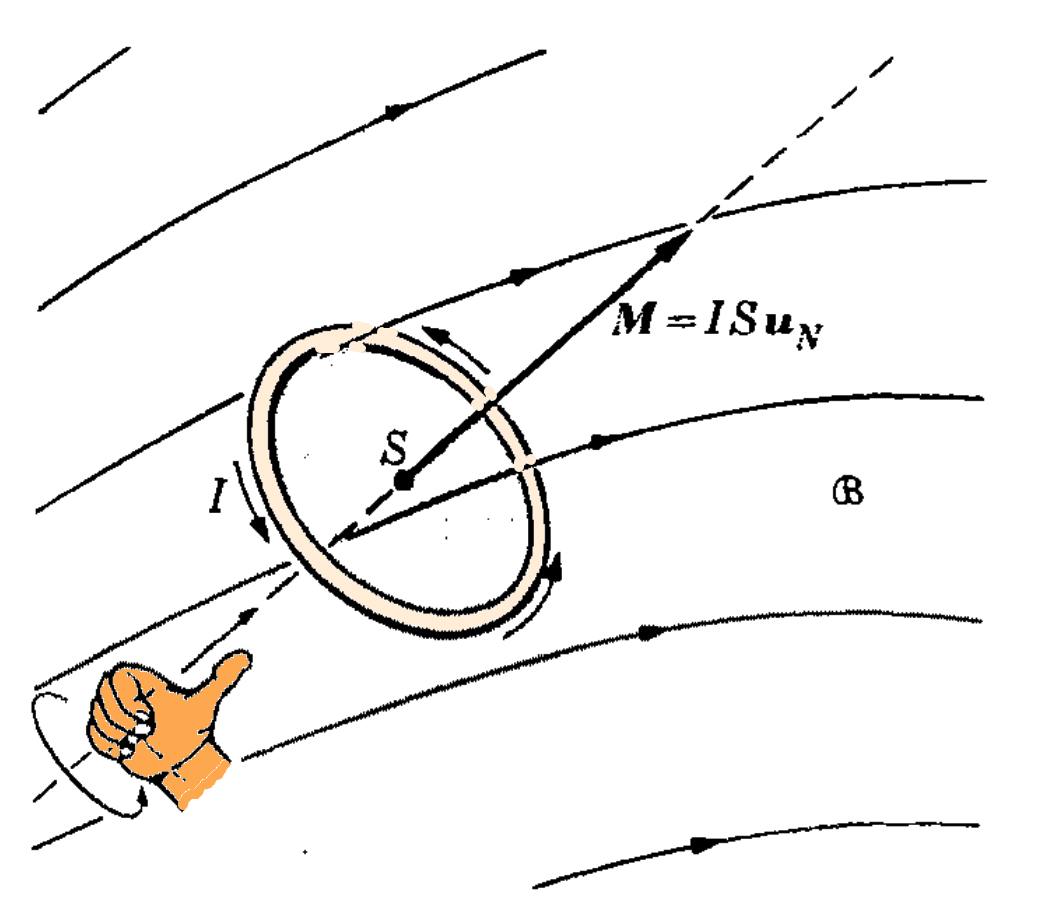
\includegraphics[width=.4\textwidth]{imagenes/imagenes26/T26IM16.png}
	\end{figure}
\end{multicols}

\section{Momento de una carga en movimiento}

Supongamos una partícula que viaja con velocidad $\vec v$ en un lugar del espacio en que existe un campo magnético $\vec B$. Nuestro problema es encontrar la trayectoria que describirá la partícula.

En cada punto de la trayectoria, la particula se encuentra sometida a la fuerza de Lorents, $\ \vec F=q\vec v \times \vec B = \displaystyle m \dv{\vec v}{t}$

Condiciones iniciales: $\ \vec B; \ \vec v,\ q$

\underline{\emph{Caso particular}}: $\boldsymbol{ \ \vec B}\ $ uniforme y $\ \boldsymbol{\vec v \ \bot \ \vec B}$

$\ \vec F=q\vec v \times \vec B = qvB\ \vec u_p$, con $\vec u_p$ unitario y perpendicular al plano $\vec v - \vec B$ 

Como $\vec F \ \bot \ \vec v,\ \vec F \cdot \vec v=0$

$0=\vec F \cdot \vec v=\displaystyle m\dv{\vec v}{t} \cdot \vec v= \ \textcolor{gris}{(\vec v \cdot \dd \vec v=v\ \dd v)}\ =m \dv{v}{t} v $

Luego $\ \displaystyle \dv{t} (v^2)=0 \to v=cte\ $ por lo que \emph{el movimiento es circular}.

Si se conserva la masa, se conservará la energía cinética: $\ m \dfrac {v^2}{r}=qvB$

\begin{equation}
\subrayado{ \  \boldsymbol{ r\ = \ \dfrac{m\ v}{q\ B} } \ } 	
\qquad \qquad  
\subrayado{ \  \boldsymbol{ \omega=\dfrac{q\ B}{m} } \ }
\end{equation}

$\vec a=\vec \omega \times \vec v \to \vec F =m\vec a=m \vec \omega \times \vec v=q\vec v \times \vec B = - q \vec B \times \vec v$, hemos cambiado el signo en el último producto vectorial (anticonmutativo), de ahí el cambio en el signo.

Identificando, obtenemos:

\begin{equation}
\subrayado{ \  \boldsymbol{ \vec \omega \ = \ - \dfrac q m \ \vec B } \ } 	
\end{equation}

Si la partícula está cargada positivamente, debido al signo menos, el sentido de giro de la partícula será contraria al campo. Si está cargada positivamente, $\vec \omega$ llevará el mismo sentido que el campo.

Este fenómeno permitió a \emph{Andersen} descubrir el \emph{positrón}. Misma curvatura que el electrón pero sentido de giro contrario.

\vspace{10mm}%************************************************
\begin{multicols}{2}
	\small{?`Qué ocurre si la velocidad del cuerpo cargado tiene alguna componente en la dirección del campo pero no es exactamente paralela a él? El cuerpo se verá forzado a tomar un camino curvo pero la componente de su movimiento a lo largo del campo no cambiará. Por lo tanto la partícula describirá una trayectoria \emph{helicoidal}. Si el cuerpo inicialmente se mueve exactamente paralelo al campo magnético, no habrá ningún tipo de fuerza deflactora ya que $v_\bot$ es cero.}
\begin{figure}[H]
	\centering
	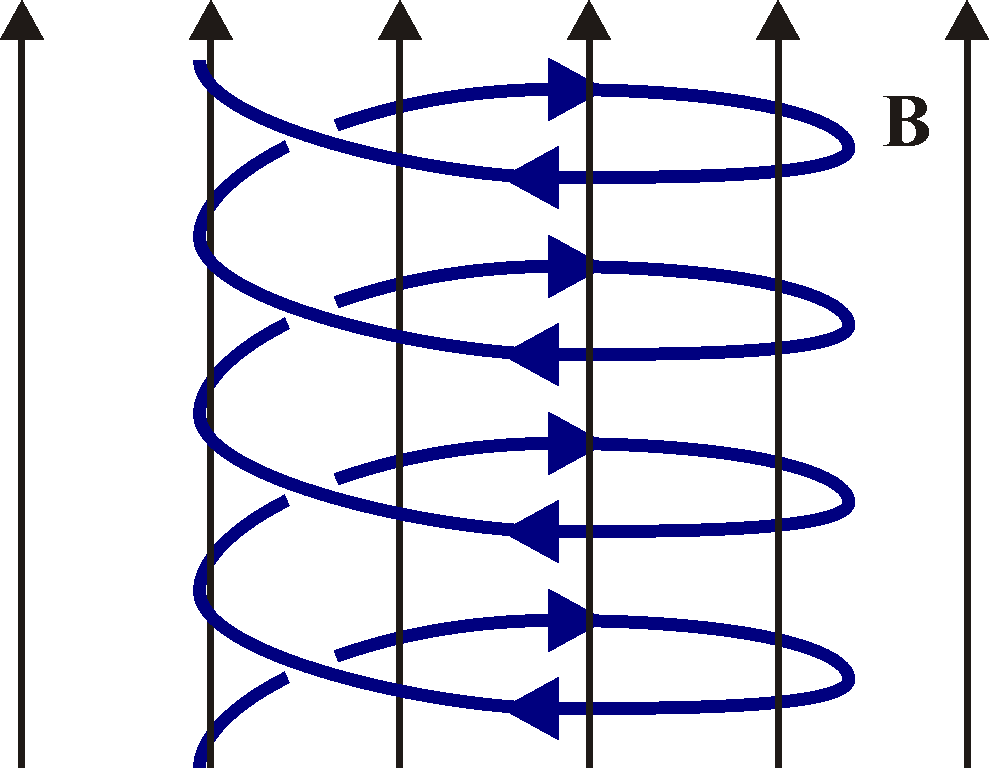
\includegraphics[width=.3\textwidth]{imagenes/imagenes26/T26IM17.png}
	\end{figure}
\end{multicols}	

\vspace{10mm}%************************************************

\begin{multicols}{2}
\small{Encontramos ejemplos de trayectorias de partículas cargadas en campos magnéticos en muchos instrumentos físicos, desde aceleradores como el LHC a cámaras de burbujas, como en fenómenos naturales como los cinturones de radiación de van Allen.}
\begin{figure}[H]
	\centering
	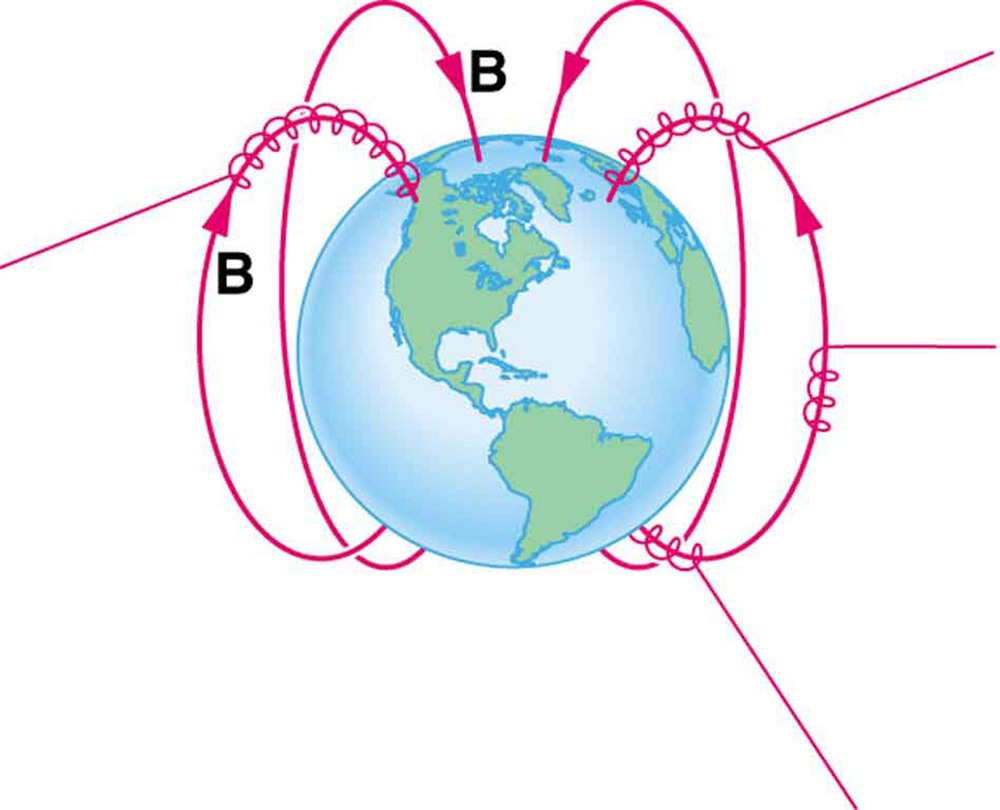
\includegraphics[width=.35\textwidth]{imagenes/imagenes26/T26IM18.png}
	\end{figure}
\end{multicols}
\begin{multicols}{2}
\small{Estos cinturones son regiones con forma de rosquilla que circundan la Tierra y que se extienden desde unos pocos cientos de kilómetros sobre la superficie terrestre hasta unos cincuenta mil kilómetros. Existe un haz continuo de partículas cargadas, la mayoría procedentes del Sol pero también del espacio exterior, que bombardean la Tierra. Muchas de estas partículas terminan siguiendo trayectorias helicoidales provocadas por el campo magnético de la Tierra y terminan atrapadas en el campo terrestre. Las partículas atrapadas se mueven en espirales hacia los polos magnéticos. Cuando alcanzan la atmósfera, excitan los átomos de los gases de ésta, que comienzan a emitir luz. Esta es la causa de las auroras.}

\small{Como los imanes actúan sobre las corrientes y las corrientes actúan sobre las corrientes, las fuerzas producidas por imanes y corrientes pueden usarse para producir trabajo haciendo que empujen o atraigan los elementos portadores de las corrientes sobre las que actúan. El uso de esta capacidad dio lugar a la aparición del motor eléctrico y el generador de electricidad, dispositivos ambos que fueron críticos en el comienzo de la era eléctrica en el XIX. El conocimiento de las trayectorias de las partículas cargadas en un campo magnético permitió el desarrollo de la física de partículas en el siglo XX, que aún continúa.}
\begin{figure}[H]
	\centering
	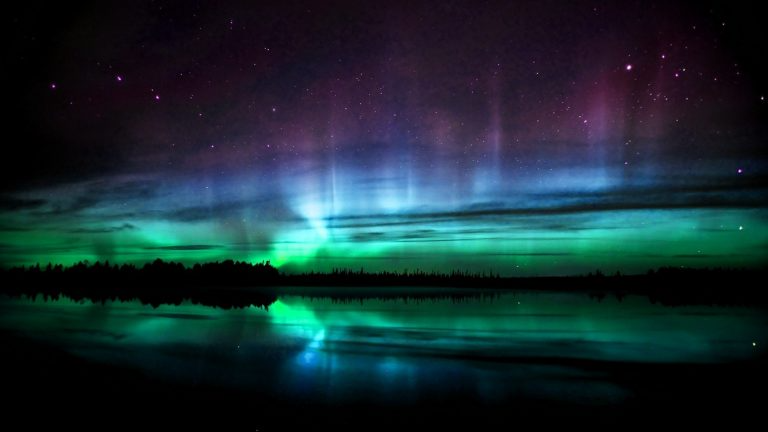
\includegraphics[width=.4\textwidth]{imagenes/imagenes26/T26IM19.png}
	\end{figure}
\end{multicols}	

\footnotesize{Artículo de \emph{César Tomé López}, extraído de `https://culturacientifica.com',  ``trayectorias de las partículas cargadas en un campo magnético''}\normalsize{.}

\section{Problemas}
	
\vspace{10mm} %***********************************************
\begin{prob}
Se hace pasar una corriente por un resorte vertical de cuyo extremo cuelga una masa $m$. ?`Qué ocurrirá?	
\end{prob}

\begin{multicols}{2}
Al circular una intensidad $I$ por el resorte, en cada espira del mismo aparecerá una fuerza magnética repulsiva entre puntos diametralmente opuestos por circular por ellos corrientes en distintos sentidos.

Al mismo tiempo, para espiras consecutivas aparcera una fuerza magnética atractiva al circular por ellas corrientes del mismo sentido.
\begin{figure}[H]
	\centering
	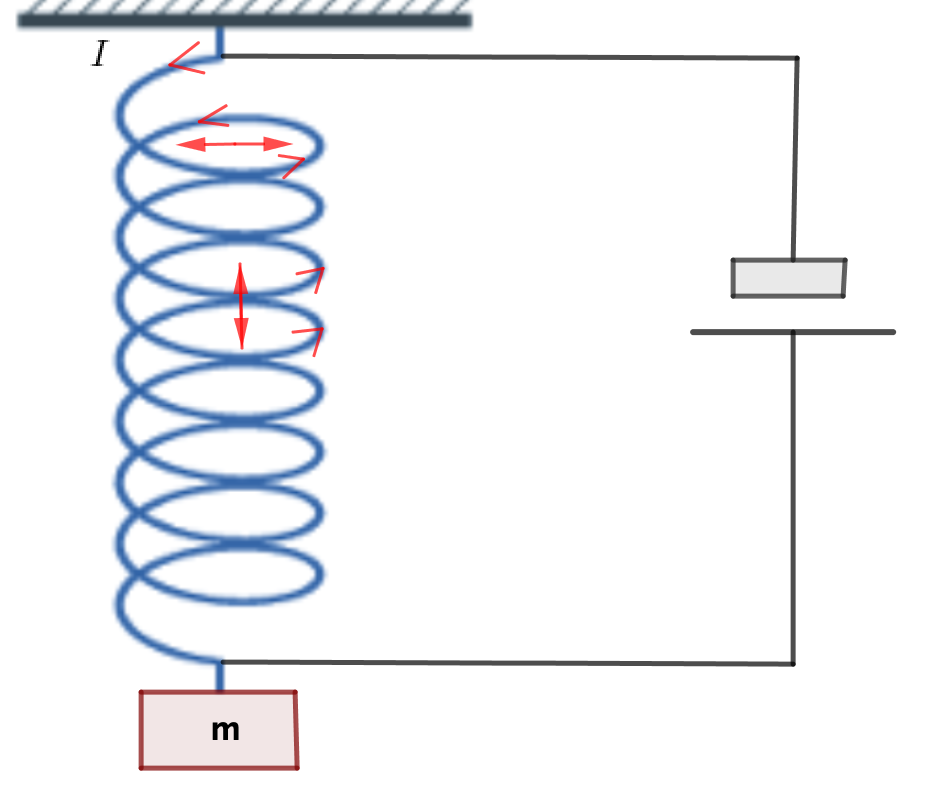
\includegraphics[width=.4\textwidth]{imagenes/imagenes26/T26IM20.png}
	\end{figure}	
\end{multicols}
\vspace{-3mm} Ambos efectos harán que el muelle se contraiga y la masa colgante subirá hacia arriba.


\vspace{10mm} %***********************************************
\begin{prob}
Un alambre en forma de U, de masa $l$ y longitud $l$ se coloca con sus dos extremos en mercurio. El alambre se encuentra en un campo magnético homogéneo $B$. Si se 	manda por el alambre un impulso de corriente $\displaystyle q=\int_0^{\Delta t} I \dd t$, el alambre salta.

Conociendo la altura $h$ que alcanza el alambre, calcular la magnitud de la carga suponiento que el tiempo $\Delta t$ que dura el impulso de la corriente es muy pequeño comparando con el tiempo de vuelo.

Caso particular: $\ m=10\ \mathrm{g}; \ l=20 \ \mathrm{cm}, \ h=3 \mathrm{m},\ B=0.1 \ \mathrm{\text{tesla}}$ 
\end{prob}

\begin{multicols}{2}
$B$ perpendicular a la imagen y dirigido hacia el lector.
$\ |\vec F_1|=|\vec F_2|$, el alambre se ensanchará.

$\vec F=\displaystyle \dv{\vec p}{t} \to \vec p=\int \vec F \dd t= \int_0^{\Delta t} I(\vec l \times \vec B)\dd t=(\vec l \times \vec B) \int_0`{\Delta t} I \dd t = \textcolor{gris}{ \ (\vec l \ \bot \ \vec B) \ }= l B \vec k q$

$p=lBq$

$\mathcal E_c=\mathcal E_p \to  \dfrac 1 2 \dfrac {p^2}m=\dfrac{1}{2}\dfrac{l^2B^2q^2}{m}=mgh$


$q=\dfrac {m}{Bl} \sqrt{2 g h} \to \text{datos:}\ q=3.83\ \mathrm{C}$
\begin{figure}[H]
	\centering
	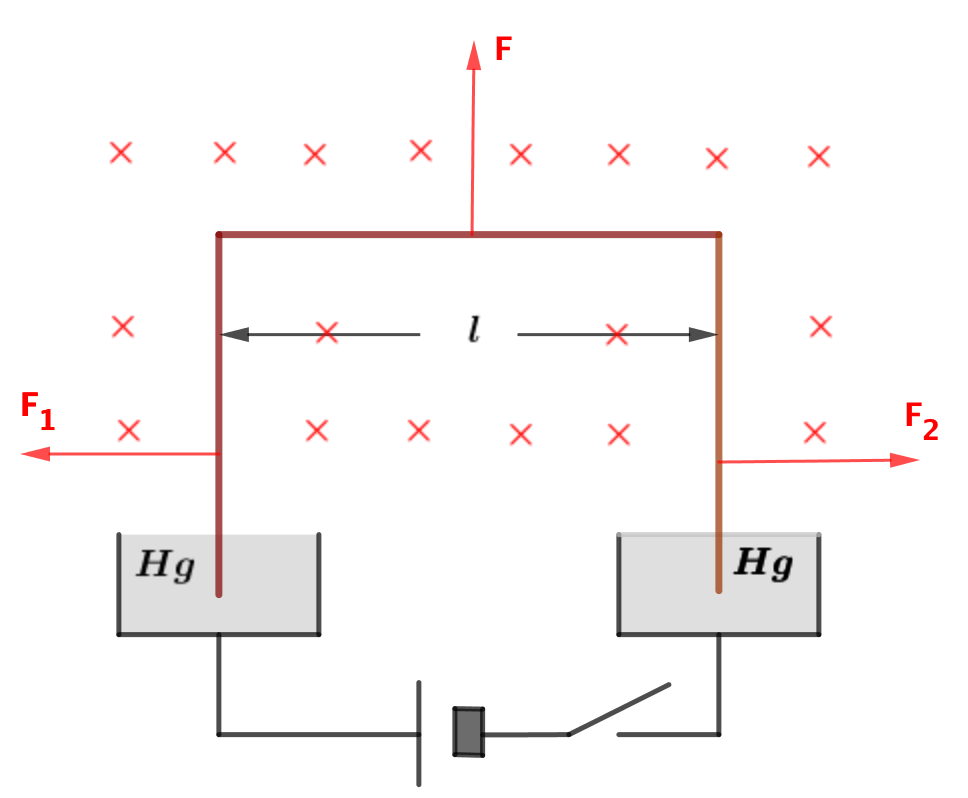
\includegraphics[width=.5\textwidth]{imagenes/imagenes26/T26IM21.png}
	\end{figure}	
\end{multicols}
	

%\begin{comment}
\newpage %********************************************
\begin{myblock}{Fuentes de campo magnético}
	%\begin{figure}[H]
	%\centering
	%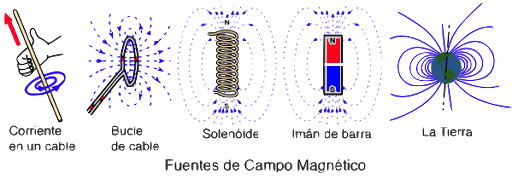
\includegraphics[width=1\textwidth]{imagenes/imagenes26/T26IM30.png}
	%\end{figure}
	
	\begin{figure}[H]
	\centering
	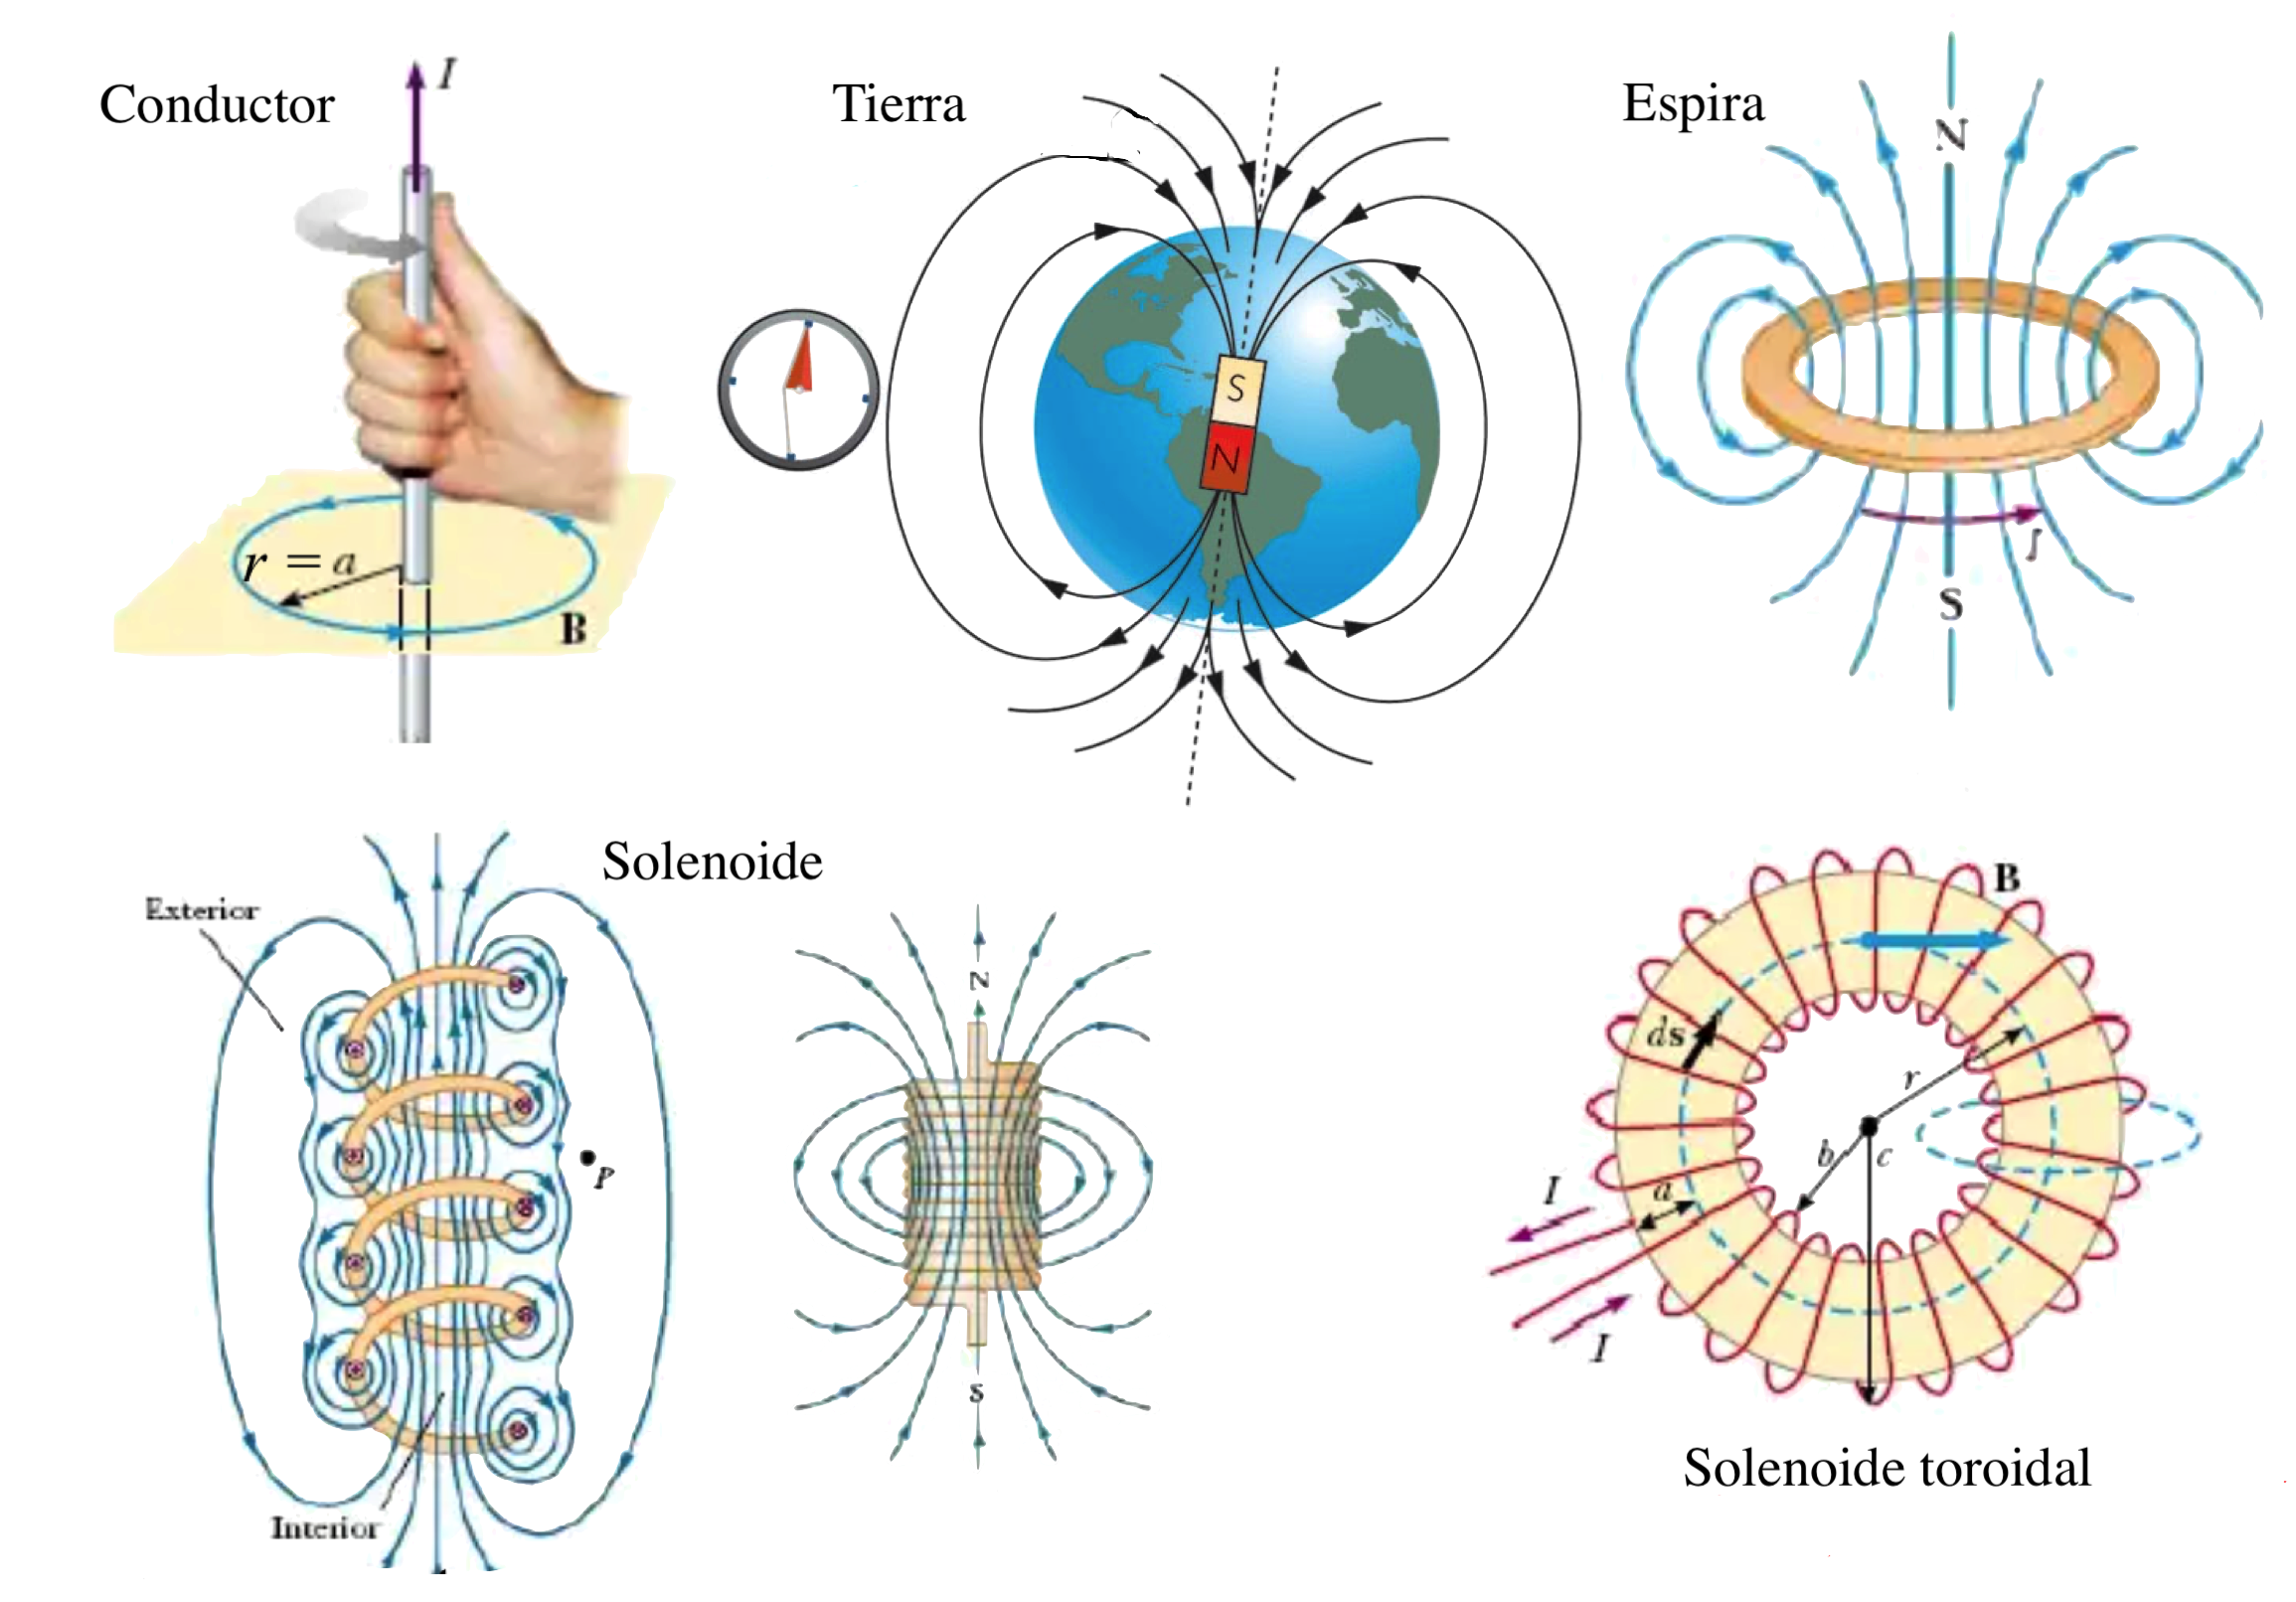
\includegraphics[width=1\textwidth]{imagenes/imagenes26/T26IM32.png}
	\caption*{Líneas de campo magnético}
	\end{figure}
	
	
	\begin{figure}[H]
	\centering
	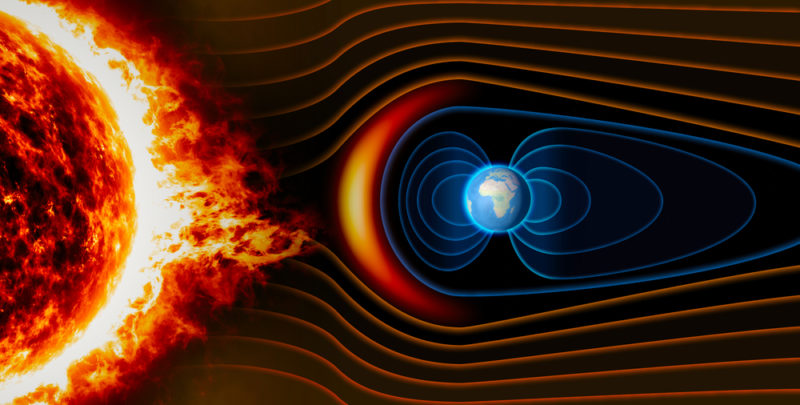
\includegraphics[width=1\textwidth]{imagenes/imagenes26/T26IM31.png}
	\caption*{Campo magnético terrestre}
	\end{figure}

\end{myblock}
%\end{comment}